\setchapterpreamble[u]{\margintoc}

\chapter{Sucesiones de Mayer-Vietoris}\labch{MVTema}
\section{Espacios de Mayer-Vietoris}
Dado un espacio topológico $X$ y una familia de subconjuntos $\mc{U}=
\{U_\alpha\colon \alpha \in A\}$ de $X$, definimos
\[\mathring{\mc{U}}=\{\mathring{U}: U \in \mc{U}\}\]
Diremos que un par $(X,\mc{U})$ es un \textbf{espacio de Mayer-Vietoris}
si $\mathring{\mc{U}}$ es un recubrimiento de $X$.

Sea $(X,\mc{U})$ un espacio de Mayer-Vietoris y $A \subseteq X$. Diremos
que $\phi\colon \sigma_n \to X$ es un $\mc{U}$-símplice si $\phi(\sigma_n)
\subset U$ para algún $U \in \mc{U}$. Dado un $n > 0$, definimos el grupo
$S^\mc{U}_n(X)$ como el subgrupo de $S_n(X)$ generado por los
$\mc{U}$-símplices de $X$. Si $\phi$ es un $\mc{U}$-símplice y $0
\leq i \leq n$, observamos que
\[\p_{(i)}\phi(\sigma_{n-1}) \subseteq \phi(\sigma_n)\]
por lo que las caras de un $\mc{U}$-símplice son de nuevo
$\mc{U}$-símplices y $S^\mc{U}_*(X)$ es un subcomplejo de cadenas de
$S_*(X)$. Además, la inclusión $i\colon S^\mc{U}_*(X) \hookrightarrow
S_*(X)$ es claramente una aplicación de cadenas.

\marginnote[-2.2cm]{
\begin{kaobox}[frametitle=Subcomplejo de cadenas]
Sea $C=(C,d)$ un complejo de cadenas. Un subcomplejo de cadenas de $C$
es un subgrupo graduado $C' \leq C$ tal que $d_n(C'_n) \leq C'_{n-1}$
para todo $n$.
\end{kaobox}
}

Sea $(Y,\mc{V})$ otro espacio de Mayer-Vietoris. Una aplicación $f\colon
(X,\mc{U}) \to (Y,\mc{V})$ es una \textbf{aplicación de Mayer-Vietoris} si,
dado un $U \in \mc{U}$, existe un $V \in \mc{V}$ tal que $f(U) \subseteq V$.
Si $f$ es una aplicación de  Mayer-Vietoris y $\phi$ es un $\mc{U}$-símplice,
existirá un $V \in \mc{V}$ tal que $f_\#(\phi)(\sigma_p) \subseteq V$,
por lo que $f$ induce una aplicación de cadenas
\[f_\#\colon S^\mc{U}_*(X) \to S^\mc{V}_*(Y)\]

\begin{theorem}[\cite{Vick94}, Apéndice I]\labthm{IncIso}
Sea $(X,\mc{U})$ un espacio de Mayer-Vietoris. La aplicación $i_*\colon
H_n(S_n^\mc{U}(X)) \to H_n(X)$ es un isomorfismo.
\end{theorem}

Sea $\mc{U}=\{U,V\}$. Si denotamos como $A$ (resp. $B$) al conjunto de
$n$-símplices singulares sobre $U$ (resp. $V$),
\begin{align*}
S_n(U)=F(A);	&& 	S_n(X)=F(A\cup B);\\
S_n(V)=F( B);	&&	S_n(U\cap V)=F(A \cap B)
\end{align*}

Consideremos las aplicaciones $g\colon F(A\cap B) \to F(A)\oplus F(B)$ y
$h\colon F(A)\oplus F(B) \to F(A\cup B)$ dadas por
\begin{align*}
g(\alpha)=(\alpha,-\alpha); && h(\alpha,\beta)=\alpha+\beta
\end{align*}
Es fácil ver que $g$ es inyectivo y $h$ es sobreyectivo.

\begin{proposition}
La secuencia
\[0 \longrightarrow S_n(U \cap V) \xrightarrow{ g } S_n(U)\oplus S_n(V)
\xrightarrow{ h } S_n^\mc{U}(X) \longrightarrow 0\]
es una sucesión exacta corta.
\end{proposition}

\begin{proof}
Por un lado, dado $c\in F(A\cap B)$,
\[(h\circ g)(c)=h(c,-c)=0\]
por lo que $\im g \leq \im h$. Por otro lado, como $h$ es sobeyectivo,
existen $a \in F(A)$ y $b \in F(B)$ tales que
\[0=h(a,b)=a+b \iff a=-b \in F(B)\]
Esto implica que $a \in F(A\cap B)$ y
\[(a,b)=(a,-a)=g(a)\]
por lo que $\ker k \leq \im g$.
\end{proof}

Definimos $S_*(U)\oplus S_*(V):=\{S_n(U)\oplus S_n(V)\colon
n \in \mb{Z}\}$, de forma que la sucesión exacta anterior da lugar a la
sucesión exacta
\[0 \longrightarrow S_*(U \cap V) \xrightarrow{ g } S_*(U)\oplus S_*(V)
\xrightarrow{ h } S^\mc{U}_*(X) \longrightarrow 0\]

Vamos a aplicar el \refthm{SucExacHomo} para obtener una sucesión exacta
en homología a partir de esta sucesión exacta corta. Para ello, observamos
que
\[H_n(S_*(U)\oplus S_*(V))\cong H_n(S_*(U))\oplus H_n(S_*(V))\cong
H_n(U)\oplus H_n(V)\]
Además, el teorema \refthm{IncIso} nos dice que $H_n(S^\mc{U}_*(X)) \cong
H_n(X)$.

\begin{definition}
Sea $(X,\mc{U})$ un espacio de Mayer-Vietoris con $\mc{U}=\{U,V\}$. Si
$\Delta\colon H_*(X) \to H_*(U \cap V)$ es el homomorfismo de conexión,
se define la \textbf{sucesión de Mayer-Vietoris} asociada a $\mc{U}$ como
la sucesión exacta
\[H_n(U \cap V) \xrightarrow{ g_* } H_n(U)\oplus H_n(V)
\xrightarrow{ h_* } H_n(X) \xrightarrow{ \Delta } H_{n-1}(U \cap V)\]
\end{definition}

El siguiente resultado establece una condición suficiente para saber
cuándo dos $1$-símplices singulares son homólogos.

\begin{lemma}
Dados dos lazos homotópicos $f,g\colon [0,1] \to X$, $[f]=[g]$.
\end{lemma}

\begin{proof}
Como sabemos por el \refexample{Camino1ciclo}, $f$ y $g$ se identifican
con $1$-ciclos de $X$ por ser caminos cerrados, por lo que $f,g \in Z_1(X)$.
Sean
\[F\colon f \simeq g\]
y $\sim$ la relación de equivalencia dada por $(t,0) \sim (t,1)$ con $t \in
[0,1]$. El espacio cociente $C=[0,1]^2/\sim$ describe un cilindro plano.

Consideremos la aplicación $F_C\colon C \to X$ inducida por $F$. Podemos
identificar $F$ con $F_C$, dado que $f$ y $g$ son lazos. Dividimos $C$ en dos
símplices orientados $c_1$ y $c_2$, como se muestra en la
\reffig{CilindroSimplices}.

\begin{marginfigure}
\resizebox{\textwidth}{!}{
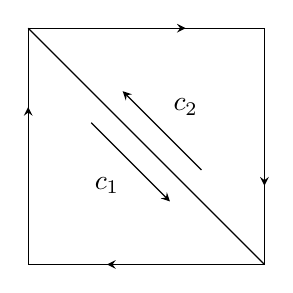
\begin{tikzpicture}
\draw (0,0) -- (0,3) -- (3,3) -- (3,0) -- cycle;

\draw[-stealth] (0,1) -- (0,2);
\draw[-stealth] (1,3) -- (2,3);
\draw[-stealth] (3,2) -- (3,1);
\draw[-stealth] (2,0) -- (1,0);

\draw (1,1) node {$c_1$};
\draw (2,2) node {$c_2$};

\draw (3,0) -- (0,3);
\draw[-stealth] (1-1/5,2-1/5) -- (2-1/5,1-1/5);
\draw[stealth-] (1+1/5,2+1/5) -- (2+1/5,1+1/5);
\end{tikzpicture}
}
\labfig{CilindroSimplices}
\caption{$C$ queda dividido en dos triángulos, $A$ y $B$, a los cuales
asignamos orientaciones contrarias.}
\end{marginfigure}

Sean $\alpha,\beta\colon \sigma_2 \to C$ los símplices singulares
\begin{align*}
\alpha(t_0,t_1,t_2)=[(t_0,t_1)]; && \beta(t_0,t_1,t_2)=[(t_0+t_1,t_0+t_2)]
\end{align*}
Usando que $(t,0)\sim (t,1)$,
\begin{align*}
\p(\beta-\alpha)(t_0,t_1)&=[(1,t_0)]-[(0,t_0)]+[(t_0,0)]-[(t_0,0)]=\\
						&=[(1,t_0)]-[(0,t_0)]
\end{align*}

Si ahora consideramos $F_\#\colon S_*(C) \to S_*(X)$,
\begin{align*}
\p [F_\#(\beta-\alpha)](t_0,t_1)=&F_\#[\p(\beta- \alpha)](t_0,t_1)=\\
                                       =&F(1,t_0)-F(0,t_0)=f(t_0)-g(t_0)
\end{align*}
Dado que $F_\#(\beta-\alpha)=F_\#(\beta)-F_\#(\alpha)$ es un 2-símplice
singular de $X$, se deduce que $f-g \in B_1(X)$. Por tanto, $f$ y $g$ son
caminos homólogos.
\end{proof}

\section{Grupo de homología de $S^1$}
Sean $U=S^1\backslash\{(1,0)\}$ y $V=S^1\backslash\{(-1,0)\}$. El espacio
$U\cap V$ es la unión disjunta de dos arcos de circunferencia, $C_1$ y $C_2$,
que son conjuntos arcoconexos. Aplicando la \refprop{SumaDirArco},
\[H_n(U\cap V) \cong H_n(C_1)\oplus H_n(C_2)\]
para todo $n \geq 0$.

En particular, el espacio puntual es un retracto por deformación fuerte de
$C_1$ y $C_2$. Usando el corolario \ref{RDFHomo} y el axioma de la dimensión,
\[H_n(C_1)\cong H_n(C_2)\cong H_n(\{\star\})\cong
\begin{cases}
\mb{Z} & \text{ si $n=0$}\\
0 & \text{ si $n\neq0$}
\end{cases}\]
Por otro lado, $U$ y $V$ son arcos de circunferencia, por lo que el mismo
razonamiento nos lleva a que
\[H_n(U)\cong H_n(V) \cong
\begin{cases}
\mb{Z} & \text{ si $n=0$}\\
0 & \text{ si $n\neq0$}
\end{cases}\]

Consideremos el siguiente tramo de la sucesión de Mayer-Vietoris asociada a
este recubrimiento:
\begin{diag}
H_1(U)\oplus H_1(V) \arrow{r}{h_1} \arrow{d}{\cong} &
H_1(S^1) \arrow{r}{\Delta_1} \arrow{d}{\cong} &
H_0(U \cap V) \arrow{d}{\cong}\\
0\arrow{r}	&H_1(S^1) \arrow{r}	&\mb{Z}^2
\end{diag}

Como la sucesión es exacta, $\im h_1=0$, luego $\ker_1 \Delta = \im h_1=0$, de
forma que $\Delta$ es un monomorfismo. Se sigue que
\[H_1(S^1)\cong \im \Delta = \ker g_1 \leq H_0(U\cap V)\cong \mb{Z}^2\]

Como $H_1(S^1) \cong \ker g_*$, podemos calcular dicho grupo estudiando cómo se
comporta el homomorfismo $g_*$.

Sea $w \in Z_0(U \cap V)$ y $[w]$ su clase módulo $B_0(U \cap V)$. Existirán
$x,y \in U \cap V$, uno en cada componente conexa, y $a,b \in \mb{Z}$ tales que
$[w]=[ax+by]$. Considérense las aplicaciones inclusión
\begin{align*}
i_*\colon H_0(U \cap V) \hookrightarrow H_0(U); &&
j_*\colon H_0(U \cap V) \hookrightarrow H_0(V)
\end{align*}
Si $[w] \in \ker g_*$, se tiene que
\[0=g_*([w])=(i_*([w]),-j_*([w])) \iff
\begin{cases}
i_*([w])=0\\
j_*([w])=0
\end{cases}\]
Pero $i_*([w]) \in H_0(U)$, por lo que $i_*([x])$ es homólogo a $i_*([y])$ y
\[0=i_*([ax+by])=i_*([ax+bx])=(a+b)i_*([x]) \iff a+b=0\]
De aquí se tiene entonces que los elementos de $\ker g_*$ son de la forma
$[ax-ay]$ con $a \in \mb{Z}$. Por tanto,
\[H_1(S^1) =\ker g_*=\la[x-y]\ra \cong \mb{Z}\]

Sea $n > 1$. Se tiene la sucesión exacta
\begin{diag}
H_n(U)\oplus H_n(V) \arrow{r}{h_n} \arrow{d}{\cong}	&
H_n(S^1) \arrow{r}{\Delta_n} \arrow{d}{\cong}&
H_{n-1}(U \cap V) \arrow{d}{\cong}\\
0\arrow{r}	&H_n(S^1) \arrow{r}	& 0
\end{diag}

Como esta sucesión es exacta, $\ker \Delta_n=\im h_n=0$. Por el primer teorema
de isomorfia,
\[H_n(S^1) \cong \frac{H_n(S^1)}{0}=\frac{H_n(S^1)}{\ker \Delta_n} \cong
\im \Delta_n=0\]

\begin{theorem}\labthm{HomoS1}
\begin{align*}
H_n(S^1)\cong
\begin{cases}
\mb{Z}&\mbox{ si }n < 2\\
0     &\mbox{ si }n \geq 2
\end{cases}
&&
\beta_n(S^1)=
\begin{cases}
1 &\mbox{ si }n < 2\\
0 &\mbox{ si }n \geq 2
\end{cases}
\end{align*}
\[\mc{X}(S^1)=1-1=0\]
\end{theorem}

Habíamos visto en el \refexample{Deformacion} que $S^1$ es una deformación de
$D^2$ y un retracto de $D^2\backslash \{(0,0)\}$. En general, esto es válido
para cualquier $p \in (D^2)^o$, no sólo para $p=(0,0)$, pero $S^1$ \textbf{no}
es un retracto de todo $D^2$.

Supongamos que existe un retracto $r\colon D^2 \to S^1$: todo retracto induce
un epimorfismo $r_*: H_1(D^2) \to H_1(S^1)$ en homología. El grupo $H_1(D^2)$
es 0 porque $D^2$ es un conjunto convexo, y acabamos de ver que $H_1(S^1)$
tiene rango 1. Dado que $r_*$ es un epimorfismo, si llamamos $\alpha$ al
generador de $H_1(S^1)$, existirá un $b \in H_1(D^2)$ tal que $r_*(b)=\alpha$.

Dado que $b \in H_1(D^2)=0$, $b=0$, por lo que $\alpha=r_*(b)=0$. Pero eso es
imposible, ya que $\alpha$ es el generador de un grupo no trivial. Por tanto,
no existen retracciones de $D^2$ en $S^1$.

\subsection{Grupo de homología de $S^n$}
La $n$-esfera se define como el conjunto $S^n\subset \mb{R}^{n+1}$ de puntos
$x$ tales que $\|x\|^2=1$. Si $\mc{N}=(0,\dots,0,1)$ y $\mc{S}=
(0,\dots,0,-1)$, consideramos el recubrimiento dado por $U=S^n\backslash
\mc{N}$ y $V=S^n\backslash \mc{S}$.

Podemos ver $S^{n-1}$ como el ecuador de $S^n$ (i.e. el subespacio de $S^n$
dado por $x_{n+1}=0$), en cuyo caso la inclusión $i\colon S^{n-1}
\hookrightarrow U\cap V$ es una equivalencia de homotopía y
\[H_*(U\cap V)\cong H_*(S^{n-1})\]
Por otro lado, $U$ y $V$ son contractos retráctiles, por lo que tienen el
tipo de homología de un punto.

Supongamos por hipótesis de inducción que, para $n-1 \geq 1$,
\[H_m(S^{n-1})\cong
\begin{cases}
\mb{Z}&\text{ si $m =0,n-1$}\\
0     &\text{ si no}
\end{cases}\]

Consideremos el siguiente tramo de la sucesión de Mayer-Vietoris:
\begin{diag}
H_n(U)\oplus H_n(V) \arrow{r}{h_n} & H_n(S^n) \arrow{d}{\Delta_n} &\\
& H_{n-1}(U\cap V) \arrow{r}{g_n} & H_{n-1}(U)\oplus H_{n-1}(V)
\end{diag}
Esta sucesión es equivalente a
\begin{diag}
0 \arrow{r} & H_n(S^n) \arrow{r}{\Delta_n} & H_{n-1}(S^{n-1}) \arrow{r} & 0
\end{diag}
de donde se sigue que $\ker \Delta_n=0$ y $H_n(S^n)\cong \im \Delta_n=
H_{n-1}(S^{n-1})$.

Para $m > n$, el tramo
\begin{diag}
H_m(U)\oplus H_m(V) \arrow{r}{h_m} & H_m(S^n) \arrow{r}{\Delta_m} &
 H_{m-1}(U\cap V)
\end{diag}
es equivalente a
\begin{diag}
0 \arrow{r} & H_m(S^n) \arrow{r}{\Delta_m} & 0
\end{diag}
por lo que $\ker\Delta_m=0=\im\Delta_m$ y $H_m(S^n)=0$.

Para $m=1$, 
\begin{diag}
H_1(U)\oplus H_1(V) \arrow{r}{h_n} & H_1(S^n) \arrow{d}{\Delta_1} &
 H_0(S^n) \arrow{r} & 0\\
& H_{0}(U\cap V) \arrow{r}{g_0} & H_{0}(U)\oplus H_{0}(V) \arrow{u}{h_0}
\end{diag}
es equivalente a
\begin{diag}
0 \arrow{r} & H_1(S^n) \arrow{r}{\Delta_m} & \mb{Z} \arrow{r}{g_0} &
\mb{Z}^2 \arrow{r}{h_0} & \mb{Z} \arrow[r] &0
\end{diag}
Usando exactitud, tenemos que
\begin{align*}
\mb{Z} \cong \im h_0 \cong \frac{\mb{Z}^2}{\ker h_0} \implies &
\ker h_0\cong \mb{Z};\\
\mb{Z} \cong \ker h_0=\im g_0\cong \frac{\mb{Z}}{\ker g_0} \implies & 
\ker g_0=0
\end{align*}
por lo que
\[H_1(S^n) \cong \frac{H_1(S^n)}{\ker \Delta_1}\cong \im \Delta_1=\ker g_0=0\]

Supongamos que $n > 2$: para $n > m > 1$,
\begin{diag}
H_m(U)\oplus H_m(V) \arrow{r}{h_m} & H_m(S^n) \arrow{r}{\Delta_m} &
H_{m-1}(U\cap V)
\end{diag}
es equivalente a
\begin{diag}
0 \arrow{r} & H_m(S^n) \arrow{r}{\Delta_m} & 0
\end{diag}
Por exactitud, $\ker \Delta_m=0=\im \Delta_m$ y $H_m(S^n)=0$. Por tanto,
\[H_m(S^n)\cong
\begin{cases}
\mb{Z}&\text{ si $m =0,n$}\\
0     &\text{ si no}
\end{cases}\]

\begin{theorem}\labthm{HomoS1}
\begin{align*}
H_m(S^n)\cong
\begin{cases}
\mb{Z}&\text{ si $m =0,n$}\\
0     &\text{ si no}
\end{cases}
&&
\beta_m(S^n)=
\begin{cases}
1 &\mbox{ si $m =0,n$}\\
0 &\mbox{ si no}
\end{cases}
\end{align*}
\end{theorem}

\section{Grupo de homología de la figura ocho}
Dados $z \in \mb{C}$, $r > 0$, sea $C(z,r)$ el conjunto de puntos $w \in
\mb{C}$ tales que $|z-w|=r$. Definimos la figura $\bm{8}$ como la unión de
las circunferencais tangentes $C(-1,1)$ y $C(1,1)$. La figura $\bm{8}$ define
un espacio de Mayer-Vietoris tomando $U,V \subset \bm{8}$ de forma que $S^1$
sea un retracto for deformación fuerte de ambos espacios (ver \reffig{ocho}).

\begin{marginfigure}
\resizebox{\textwidth}{!}{
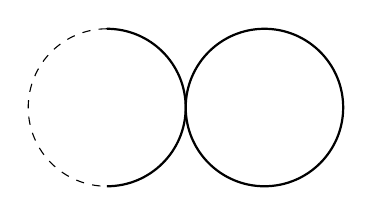
\begin{tikzpicture}
\draw[thick] (1,0) circle (1cm);
\draw[thick] (-1,-1) arc (-90:90:1);
\draw[dashed] (-1,1) arc (90:270:1);
\end{tikzpicture}
}
\caption{\labfig{ocho} Figura ocho en línea discontinua, con un posible
conjunto $U$ dibujado en línea sólida gruesa.}
\end{marginfigure}

En particular, $U\cap V$ serán dos arcos tangentes. Por construcción,
\begin{align*}
H_*(U)\cong H_*(V)\cong H_*(S^1)^2; && H_*(U\cap V)\cong H_*(\{\star\})
\end{align*}

Para $n > 1$, se tiene la sucesión exacta corta
\begin{diag}
H_n(U\cap V) \arrow{r}{g_n} \arrow{d}{\cong} &
H_n(U)\oplus H_n(V) \arrow{r}{h_n} \arrow{d}{\cong} &
H_n(\bm{8}) \arrow{r}{\Delta_n} \arrow{d}{\cong} &
H_{n-1}(U\cap V) \arrow{d}{\cong}\\
0 \arrow{r} & 0 \arrow{r} & H_n(\bm{8}) \arrow{r} & 0
\end{diag}
Por exactitud,
\[0=\im h_n\cong \frac{H_n(8)}{\ker h_n}=\frac{H_n(8)}{\im g_n}\cong H_n(8)\]

Consideremos el siguiente tramo:
\begin{diag}
H_1(U\cap V) \arrow{r}{g_1} \arrow{d}{\cong} &
H_1(U)\oplus H_1(V) \arrow{r}{h_1} \arrow{d}{\cong} &
H_1(\bm{8}) \arrow{r}{\Delta_1} \arrow{d}{\cong} &
H_0(U\cap V) \arrow{d}{\cong}\\
0 \arrow{r} & \mb{Z}^2 \arrow{r} & H_1(\bm{8}) \arrow{r} & \mb{Z}
\end{diag}
Por exactitud,
\begin{align*}
\frac{H_1(\bm{8})}{\ker \Delta_1}\cong \im \Delta_1=\ker g_0;&&
\ker \Delta_1=\im h_1 \cong \frac{\mb{Z}^2}{\ker h_1} \cong \mb{Z}^2;
\end{align*}
Es decir,
\begin{equation}
\ker g_0\cong\frac{H_1(\bm{8})}{\mb{Z}^2} \label{H1ocho}
\end{equation}

Consideremos el siguiente tramo:
\begin{diag}
H_0(U\cap V) \arrow{r}{g_0} \arrow{d}{\cong} &
H_0(U)\oplus H_0(V) \arrow{r}{h_0} \arrow{d}{\cong} &
H_0(\bm{8}) \arrow{r}{\Delta_0} \arrow{d}{\cong} &
0 \arrow{d}{\cong}\\
\mb{Z} \arrow{r} & \mb{Z}^2 \arrow{r} & \mb{Z} \arrow{r} & 0
\end{diag}
Por exactitud,
\begin{align*}
\mb{Z} \cong \ker \Delta_0=\im h_0 \cong \frac{\mb{Z}^2}{\ker h_0}
&\implies \ker h_0\cong \mb{Z}\\
\mb{Z}\cong \ker h_0=\im g_0\cong \frac{\mb{Z}}{\ker g_0} & \implies
\ker g_0=0
\end{align*}
Aplicando esta información en la ecuación \eqref{H1ocho}, concluimos que
$H_1(\bm{8})\cong \mb{Z}^2$.

\begin{theorem}
\begin{align*}
H_n(\bm{8})\cong
\begin{cases}
\mb{Z}		&\mbox{ si }n =0\\
\mb{Z}^2	&\mbox{ si }n =1\\
0     &\mbox{ si }n \geq 2
\end{cases}
&&
\beta_n(\bm{8})=
\begin{cases}
1 &\mbox{ si }n = 0\\
2 &\mbox{ si }n = 1\\
0 &\mbox{ si }n \geq 2
\end{cases}
\end{align*}
\[\mc{X}(\bm{8})=1-2=-1\]
\end{theorem}

\subsection{La rosa del topólogo}
La figura ocho se puede construir utilizando cocientes, lo que nos permite
generalizar esta construcción. Sean $p \in \mb{R}^2$ y $I \subset \mb{R}$
un intervalo cerrado y acotado. Si
\[R=\p I\sqcup \p I\sqcup \{p\}\]
la figura ocho antes descrita se puede representar como
\[\frac{I\sqcup\{p\}\sqcup I}{R}\]
Podemos extender esta construcción para añadir tantos lóbulos como queramos,
de forma que conseguimos una figura llamada \textbf{rosa} o \textbf{buqué}.

Dado un $n > 0$, se define la rosa de $n$ pétalos ($B_n$) como
\begin{align*}
J_1	&=I\sqcup \{p\}; 	& R_1	&=\{p\}\sqcup \p I;		&
B_1	&=\frac{J_1}{R_1}\cong S^1;\\
J_2	&=J_1\sqcup I;		& R_2	&=R_1\sqcup \p I; 		&
B_2	&=\frac{J_2}{R_2}\cong \bm{8};\\
	&\hdots				& 		&\hdots					&
\hdots\\
J_n	&=J_{n-1}\sqcup I;	& R_n	&=R_{n-1}\sqcup \p I;	&
B_n	&=\frac{J_n}{R_n}
\end{align*}
Esto crea una recurrencia que nos lleva a la definición de $B_n$.

Hasta ahora, sabemos que
\begin{align*}
H_n(B_1)\cong
\begin{cases}
\mb{Z}	&\mbox{ si $n =0$}\\
\mb{Z}	&\mbox{ si $n =1$}\\
0    	&\mbox{ si $n \geq 2$}
\end{cases}
&&
H_n(B_2)\cong
\begin{cases}
\mb{Z}		&\mbox{ si $n =0$}\\
\mb{Z}^2 	&\mbox{ si $n =1$}\\
0		    &\mbox{ si $n \geq 2$}
\end{cases}
\end{align*}
Conjeturamos entonces que
\[H_n(B_p)\cong
\begin{cases}
\mb{Z}		&\mbox{ si $n =0$}\\
\mb{Z}^p	&\mbox{ si $n =1$}\\
0     &\mbox{ si $n \geq 2$}
\end{cases}\]

\marginnote[-2.2cm]{
\begin{kaobox}[frametitle=Conjunto estrellado]
Un conjunto $A \subseteq \mb{R}^n$ es estrellado si existe un $a_0 \in A$ tal
que $[a_0,x] \subseteq A$ para todo $x \in A$. Un conjunto estrellado es un
punto intermedio entre un conjunto contráctil y un conjunto convexo. Típicos
ejemplos de conjuntos estrellados incluyen el símbolo asterisco y la letras
X e Y.
\end{kaobox}
}

Consideremos entonces la rosa de $p+1$ pétalos, $B_{p+1}$. Definimos el
espacio de Mayer-Vietoris donde $B_p$ es un retracto por deformación fuerte
de $U$ y $S^1$ es un retracto por deformación fuerte de $V$. Observamos que
$U\cap V$ describe un conjunto estrellado, por lo que tiene el tipo de
homología de un punto.

Para $n > 1$,

\adjustbox{scale=0.8, center}{
\begin{tikzcd}
H_n(U\cap V) \arrow{r}{g_n} \arrow{d}{\cong} &
H_n(U)\oplus H_n(V) \arrow{r}{h_n} \arrow{d}{\cong} &
H_n(B_{p+1}) \arrow{r}{\Delta_n} \arrow{d}{\cong} &
H_{n-1}(U\cap V) \arrow{d}{\cong}\\
0 \arrow{r} & 0 \arrow{r} & H_n(B_{p+1}) \arrow{r} & 0
\end{tikzcd}
}

Por exactitud, $\ker \Delta_n=0$ y $\im \Delta_n=0=H_{n-1}(U\cap V)$, por lo
que $\Delta$ es un isomorfismo. Se sigue que
\[H_n(B_{p+1}) \cong H_{n-1}(U\cap V)=0\]

\begin{marginfigure}
\resizebox{\textwidth}{!}{
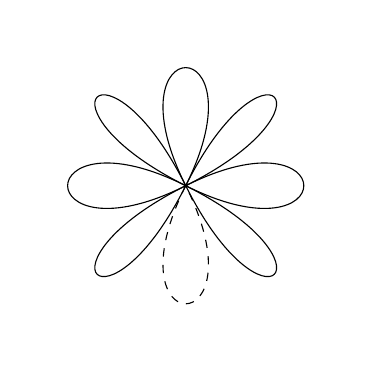
\begin{tikzpicture}
\draw (0,0) .. controls (2,1) and (1,2) .. (0,0);
\draw (0,0) .. controls (1,2) and (-1,2) .. (0,0);
\draw (0,0) .. controls (-1,2) and (-2,1) .. (0,0);
\draw (0,0) .. controls (-2,1) and (-2,-1) .. (0,0);
\draw (0,0) .. controls (-2,-1) and (-1,-2) .. (0,0);
\draw[dashed] (0,0) .. controls (-1,-2) and (1,-2) .. (0,0);
\draw (0,0) .. controls (1,-2) and (2,-1) .. (0,0);
\draw (0,0) .. controls (2,-1) and (2,1) .. (0,0);
\end{tikzpicture}
}
\caption[Rosa de 8 pétalos.]{Rosa de $8$ pétalos. La línea discontinua
representa la adición de un nuevo pétalo.}
\end{marginfigure}

Consideremos el siguiente tramo:
\begin{diag}
H_1(U\cap V) \arrow{r}{g_1} \arrow{d}{\cong} &
H_1(U)\oplus H_1(V) \arrow{r}{h_1} \arrow{d}{\cong} &
H_1(B_{p+1}) \arrow{r}{\Delta_1} \arrow{d}{\cong} &
H_0(U\cap V) \arrow{d}{\cong}\\
0 \arrow{r} & \mb{Z}^{p+1} \arrow{r} & H_1(B_{p+1}) \arrow{r} & \mb{Z}
\end{diag}
Por exactitud,
\begin{align*}
\frac{H_1(B_{p+1})}{\ker \Delta_1}\cong \im \Delta_1=\ker g_0;&&
\ker \Delta_1=\im h_1 \cong \frac{\mb{Z}^{p+1}}{\ker h_1} \cong \mb{Z}^{p+1};
\end{align*}
Es decir,
\begin{equation}
\ker g_0\cong\frac{H_1(B_{p+1})}{\mb{Z}^{p+1}} \label{H1rosa}
\end{equation}

Consideremos el siguiente tramo:
\begin{diag}
H_0(U\cap V) \arrow{r}{g_0} \arrow{d}{\cong} &
H_0(U)\oplus H_0(V) \arrow{r}{h_0} \arrow{d}{\cong} &
H_0(B_{p+1}) \arrow{r}{\Delta_0} \arrow{d}{\cong} &
0 \arrow{d}{\cong}\\
\mb{Z} \arrow{r} & \mb{Z}^2 \arrow{r} & \mb{Z} \arrow{r} & 0
\end{diag}
Por exactitud,
\begin{align*}
\mb{Z} \cong \ker \Delta_0=\im h_0 \cong \frac{\mb{Z}^2}{\ker h_0}
&\implies \ker h_0\cong \mb{Z}\\
\mb{Z}\cong \ker h_0=\im g_0\cong \frac{\mb{Z}}{\ker g_0} & \implies
\ker g_0=0
\end{align*}
Aplicando esta información en la ecuación \eqref{H1rosa}, concluimos que
\\$H_1(B_{p+1})\cong \mb{Z}^{p+1}$. Esto confirma nuestra conjetura.

\begin{theorem}
\begin{align*}
H_n(B_p)\cong
\begin{cases}
\mb{Z}		&\mbox{ si }n =0\\
\mb{Z}^p	&\mbox{ si }n =1\\
0     &\mbox{ si }n \geq 2
\end{cases}
&&
\beta_n(B_p)=
\begin{cases}
1 &\mbox{ si }n = 0\\
p &\mbox{ si }n = 1\\
0 &\mbox{ si }n \geq 2
\end{cases}
\end{align*}
\[\mc{X}(B_p)=1-p\]
\end{theorem}

\section{Grupo de homología del toro}
El \textbf{toro de Clifford} o \textbf{toro llano} se define como el espacio cociente
\[T=\frac{[0,1]^2}{\sim}\]
donde $\sim$ es la menor relación de equivalencia tal que $(t,0) \sim (t,1)$ y
$(0,t) \sim (1,t)$ para todo $t \in [0,1]$. Podemos inducir una estructura de
espacio de Mayer-Vietoris tomando los conjuntos
\begin{align*}
U=\left\{[(x,y)] \in T\colon x > \frac{1}{3} \right\}; &&
V=\left\{[(x,y)] \in T\colon y < \frac{2}{3} \right\};
\end{align*}
Los conjuntos $U$, $V$ y $U\cap V$ son cilindros, por lo que tienen el tipo
de homología de $S^1$.

\begin{marginfigure}
\resizebox{\textwidth}{!}{
\begin{tikzpicture}
\draw (0,0) -- (0,3) -- (3,3) -- (3,0) -- cycle;

%Left
\draw[-stealth] (0,0) -- (0,1);
\draw[-stealth] (0,1) -- (0,2);

%Right
\draw[-stealth] (3,0) -- (3,1);
\draw[-stealth] (3,1) -- (3,2);

%Up and down
\draw[-stealth] (1,0) -- (1.5,0);
\draw[-stealth] (1,3) -- (1.5,3);
\end{tikzpicture}
}
\labfig{Clifford}
\caption[Toro de Clifford]{Representación plana del toro de Clifford.}
\end{marginfigure}

Sea $n > 2$. Consideramos la siguiente sucesión exacta:
\begin{diag}
H_n(U\cap V) \arrow{r}{g_n} \arrow{d}{\cong} &
H_n(U)\oplus H_n(V) \arrow{r}{h_n} \arrow{d}{\cong} &
H_n(T) \arrow{r}{\Delta_n} \arrow{d}{\cong} &
H_{n-1}(U\cap V) \arrow{d}{\cong}\\
0 \arrow{r} & 0 \arrow{r} & H_n(T) \arrow{r} & 0
\end{diag}
Al igual que en los ejemplos anteriores, $H_n(T)=0$.

Para $n=0$,
\begin{diag}
H_0(U\cap V) \arrow{r}{g_0} \arrow{d}{\cong} &
H_0(U)\oplus H_0(V) \arrow{r}{h_0} \arrow{d}{\cong} &
H_0(T) \arrow{r}{\Delta_0} \arrow{d}{\cong} &
0 \arrow{d}{\cong}\\
\mb{Z} \arrow{r} & \mb{Z}^2 \arrow{r} & \mb{Z} \arrow{r} & 0
\end{diag}
Dado que esta sucesión es exacta, $\im h_0=\ker \Delta_0 \cong \mb{Z}$ y
$\im g_0=\ker h_0\cong \mb{Z}$, luego
\begin{align*}
\frac{\mb{Z}^2}{\ker h_0} \cong \im h_0 \cong \mb{Z} &\implies
\ker h_0\cong\mb{Z}\\
\frac{\mb{Z}}{\ker g_0} \cong \im g_0 \cong \mb{Z} &\implies
\ker g_0=0
\end{align*}

Pasemos a $n=1$:
\begin{diag}
H_1(U\cap V) \arrow{r}{g_1} \arrow{d}{\cong} &
H_1(U)\oplus H_1(V) \arrow{r}{h_1} \arrow{d}{\cong} &
H_1(T) \arrow{r}{\Delta_1} \arrow{d}{\cong} &
H_0(U\cap V) \arrow{d}{\cong}\\
\mb{Z} \arrow{r} & \mb{Z}^2 \arrow{r} & H_1(T) \arrow{r} & \mb{Z}
\end{diag}

Dado que la sucesión es exacta, $\im \Delta_1=\ker g_0=0$ y
\begin{equation}
\label{H1toro}H_1(T)=\ker \Delta_1=\im h_1 \cong
\frac{\mb{Z}^2}{\ker h_1}=\frac{\mb{Z}^2}{\im g_1}
\end{equation}

Pasemos a $n=2$:
\begin{diag}
H_2(U\cap V) \arrow{r}{g_2} \arrow{d}{\cong} &
H_2(U)\oplus H_2(V) \arrow{r}{h_2} \arrow{d}{\cong} &
H_2(T) \arrow{r}{\Delta_2} \arrow{d}{\cong} &
H_1(U\cap V) \arrow{d}{\cong}\\
0 \arrow{r} & 0 \arrow{r} & H_2(T) \arrow{r} & \mb{Z}
\end{diag}

Una serie de operaciones basadas en la exactitud de esta secuencia nos
lleva a que $H_2(T)\cong\ker g_1$, pero no podemos hallar $\ker g_1$ usando
sólo exactitud. Necesitamos calcular $\ker g_1$ directamente.

Por definición, $g_1\colon H_1(S^1) \longrightarrow H_1(S^1)^2$ se define como
\[g([c])=([c],[-c])\]
Sea $[c] \in \ker g_1$ y $x,y \in Z_1(S^1)$, $x\neq y$, tales que $[x]$ e
$[y]$ son generadores de $H_1(S^1)$. Notemos que $x$ e $y$ son homólogos, ya
que $H_1(S^1)$ tiene rango $1$. Existen $\alpha,\beta$ enteros tales que
\[c=\alpha x+\beta y\]
Consideramos las inclusiones $i\colon U \cap V \hookrightarrow U$ y
$j\colon U \cap V \hookrightarrow V$. Tenemos que
\[0=g_*([c])=([c],-[c])=(i_*[c],-j_*[c]) \iff \begin{cases}i_*([c])
\\
j_*([c])=0\end{cases}\]
Dado que $x$ e $y$ son homólogos,
\[i_*([c])=i_*([\alpha x+\beta y])=i_*([\alpha x+\beta x])=
(\alpha+\beta)i_*([x])=0 \iff \alpha=-\beta\]
por lo que $H_2(T)\cong \ker g_1\cong \mb{Z}$. Usando esta información,
\[\im g_1 \cong \frac{\mb{Z}}{\ker g_1}=0 \arriba{\eqref{H1toro}}{\implies}
H_1(T)\cong \mb{Z}^2\]

\begin{theorem}\label{HomoToro}
\[\begin{array}{ccc}
H_n(T)=
\begin{cases}
\mb{Z}		&\mbox{ si }n =0,2\\
\mb{Z}^2	&\mbox{ si }n =1\\
0     &\mbox{ si }n > 2
\end{cases}
&\implies&
\beta_n(T)=
\begin{cases}
1 &\mbox{ si }n = 0,2\\
2 &\mbox{ si }n = 1\\
0 &\mbox{ si }n > 2
\end{cases}
\end{array}\]
\[\mc{X}(T)=1-2+1=0\]
\end{theorem}

Más adelante veremos que se pueden hallar los grupos de homología del toro de
forma mucho más directa.
